\documentclass{notes}
\usepackage{lipsum}

% \title{Statistical Inference}
\coursetitle{Introduction to Quantum Astronomy}
\subtitle{Lecture Notes}
\coursecode{qa224}
\professor{
  Theo Von\authorhref[mailto:theovon@seas.harvard.edu]{theovon@seas}
}
\scribe{
  Matthew Nazari\authorhref[mailto:matthewnazari@college.harvard.edu]{matthewnazari@college}
  \and
  Bella Tarantino\authorhref[mailto:bellatarantino@college.harvard.edu]{bellatarantino@college}
}
\place{Harvard University}
\season{Summer}
\year{2021}
% \date{29}{6}{2021}
\begin{document}
  \section{Introduction}
  \lipsum[1-2]
  \marginpar{Note that this is a note on the margin. Margins notes are notes nonetheless.}
  \lipsum[2-3]
  \subsection{This is a subsection}
  \lipsum[3-3]
  \begin{marginfig}[This is a super cool caption]
    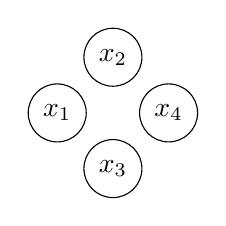
\begin{tikzpicture}[main/.style = {draw, circle}]
      \node[main] (1) {$x_1$};
      \node[main] (2) [above right of=1] {$x_2$};
      \node[main] (3) [below right of=1] {$x_3$}; 
      \node[main] (4) [above right of=3] {$x_4$};
    \end{tikzpicture}
  \end{marginfig}
  \lipsum[4-6]
  \marginpar{Oh lord, \textit{more} margin notes? This is outright preposterous! The nerve of some scribes.}
  \subsection{Introducing things still}
  \lipsum[5-6]

  \section{Astronomic approach}
  \lipsum[7-9]
  \begin{fig}[This is a super dope, and somewhat long caption.]%
      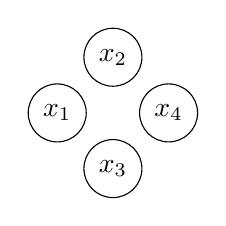
\begin{tikzpicture}[main/.style = {draw, circle}]
        \node[main] (1) {$x_1$};
        \node[main] (2) [above right of=1] {$x_2$};
        \node[main] (3) [below right of=1] {$x_3$}; 
        \node[main] (4) [above right of=3] {$x_4$};
      \end{tikzpicture}
  \end{fig}
  \lipsum[10-10]
  \begin{example}[This is an example.]
    This is a example yo!%
    \lipsum[5]
    \begin{align*}
      \int_{x=1}^{x=\infty}\max\left\{\frac12\,f(x), 0\right\}\,dx &= \sum_{n=1}^{\infty}e^{n\pi} \\
      &= e^{1\pi} + \ldots + e^{n\pi} \\
      &= \sqrt{e^{i\pi}}
    \end{align*}
    \lipsum[2]
  \end{example}
  \begin{theorem}[Theorem Name]
    In mathematics, particularly linear algebra and functional analysis, a spectral theorem is a result about when a linear operator or matrix can be diagonalized. Let $x$ be $y$ and $y$ be the first $x$ in $y$. Then
    $$\int_{x=1}^{x=\infty}\frac12\,f(x)\,dx = \pi$$%
  \end{theorem}
  \begin{proof}
    This is my proof. The end.
  \end{proof}
  \begin{lemma}[Lemma Name]
    This is a lemma yo!%
  \end{lemma}
  \begin{corollary}[Corollary Name]
    This is a corollary yo!%
  \end{corollary}
  \begin{proposition}[Proposition Name]
    This is a proposition yo!%
  \end{proposition}
  \begin{remark}[Remark title]
    This is a proposition yo!%
  \end{remark}
  \lipsum[10-10]
  \subsection{Planets, stars, moons, oh my!}
  \lipsum[11-13]
  \section{Quantum approach}
  \lipsum[14-16]
  \subsection{Tony stark and gamma rays}
  \lipsum[17-18]

\end{document}

